\documentclass[pdftex,12pt,a4paper]{article}

\usepackage{graphicx}  
\usepackage[margin=2.5cm]{geometry}
\usepackage{breakcites}
\usepackage{indentfirst}
\usepackage{pgfgantt}
\usepackage{pdflscape}
\usepackage{float}
\usepackage{epsfig}
\usepackage{epstopdf}
\usepackage[cmex10]{amsmath}
\usepackage{stfloats}
\usepackage{multirow}

\renewcommand{\refname}{REFERENCES}
\linespread{1.3}

\usepackage{mathtools}
%\newcommand{\HRule}{\rule{\linewidth}{0.5mm}}
\thispagestyle{empty}
\begin{document}
\begin{titlepage}
\begin{center}
\textbf{}\\
\textbf{\Large{ISTANBUL TECHNICAL UNIVERSITY}}\\
\vspace{0.5cm}
\textbf{\Large{COMPUTER ENGINEERING DEPARTMENT}}\\
\vspace{2cm}
\textbf{\Large{BLG 222E\\ Computer Organization \\ Project 1}}\\
\vspace{2.8cm}
\begin{table}[ht]
\centering
\Large{
\begin{tabular}{lcl}
\textbf{PROJECT DATE}  & : & 12.04.2023\\
\end{tabular}}
\end{table}
\vspace{1cm}
\textbf{\Large{GROUP MEMBERS:}}\\
\begin{table}[ht]
\centering
\Large{
\begin{tabular}{rcl}
150220762  & : & Muhammed Yusuf Mermer  \\
150210071  & : & Emre Çamlıca \\
150200091  & : & Hakan Duran \\
\end{tabular}}
\end{table}
\vspace{2.8cm}
\textbf{\Large{SPRING 2023}}

\end{center}

\end{titlepage}

\thispagestyle{empty}
\addtocontents{toc}{\contentsline {section}{\numberline {}FRONT COVER}{}}
\addtocontents{toc}{\contentsline {section}{\numberline {}CONTENTS}{}}
\setcounter{tocdepth}{4}
\tableofcontents
\clearpage

\setcounter{page}{1}
\section{INTRODUCTION}
In this project our purpose is to make arithmetic logic unit (ALU) system. To achive 
this we firstly implemented small components of this system. Hakan did the parts 1, 2.a and 2.b; 
Yusuf did the parts 2.c and 4; Emre did the part 3.

At first, we designed n-bit register which accepts any n bit binary number and make
operations as if loading incrementing and decrementing by 1 and clearing.

In the second part we desgined compenents which contain multiple registers and 
manipulated them regarding to the incoming inputs. In part 2.a, we designed
instruction Register (IR). Only one half of the register affected at a time.
In part 2.b,  we designed register file (RF). One can change any register at any time even can 
change all registers at the same time. Besides, number of output also changed. We can send
2 output for various different combinations. Then we implemented Adress Register File (ARF),
which contains program counter (PC), Adress Register (AR), Stack Pointer (SP) and PcPast.
These registers are all 8 bits, so only difference between RF and ARF is that later contains
4 of 8-bit register.  

Then we implemented ALU. It makes 16 different operations to two number. It is simply a 
combinational logic device which does not contains memory to make operations faster.
Returns 4 bit of flag whose purpose is explained in the next section.




\section{IMPLEMENTATIONS AND EXPLANATIONS }
\subsection{Part 1}
In part 1, we design a register in which will be used in other parts. Register
is n bit register. Here, n has a parameter functionality. We can adjust 
how many bits in it. This register has an enable input which adjusts 
if the register will be protect
its previous state or will change its value. 

Changing register's value is
provided by 2 bit FunSel input. FunSel has 4 different combinations for clear,
load, decrement and increment. Clear function is changing register's value to
n bit zero. Load function is loading n bit load value to register. Decrement and
increment functions changing register's value by adding or substracting one to 
previous value. Register's current value can be reached from Qout output port.

In register module, always block has been used and trigger time of always block
is when clock is at positive edge situation. Then if block checks for enable input.
If enable is 0, then nothing happens so that value of register remains same. If
enable is 1, then which function will be processed by controlling the FunSel input.

\subsubsection{}
\textbf{inputs:}    clk(1 bit),
enable(1 bit),
funsel(2 bits),
load(n bits),

\textbf{outputs:}    
Qout(n bits)

\textbf{module name:} register

\subsection{Part 2}
\subsubsection{Part 2.a}
In part 2a, we implemented instruction register (IR) which will be used in ALU System.
This register has enable input that has same functionality with part 1 register. It
is for adjusting if IR will remain same or change its value. Thsi register take 8
bit input and gives 16 bit output.

Changing IR's value is provided by 2 bit FunSel and LH input. FunSel's clear,
increment and decrement functions are doing same functions with that of part 1
register and LH input is not important for this functions. In FunSel's load function,
there is two different choices where to load input bits. We can load inputs to IR's
least significant bits (0 to 7), or most significant bits (8 to 15). The choose is
ensured by LH input.

In instruction register module, we use an always block whose trigger time is clock's
positive edge. Then if block checks for enable input.
If enable is 0, then nothing happens so that value of register remains same. If
enable is 1, then which function will be processed by controlling the FunSel 
and LH input.

\subsubsection{}
\textbf{inputs:}    clk(1 bit),
data(8 bits),
enable(1 bit),
funsel(2 bits),
lh(1 bit)

\textbf{outputs:}    
irout(16 bits)

\textbf{module name:} ir

\subsubsection{Part 2.b}
In part 2b, we implemented a register file which consists of 8 8-bit register. Half of
registers are general purpose registers: R1, R2, R3, R4. Other half of registers
are temporary registers: T1, T2, T3, T4. 

Those registers' value can be changed 
with FunSel input. To provide effectiveness of FunSel, registers should be enabled
with RSel and TSel inputs. Enabled registers are changed by FunSel and FunSel has
4 different functions. They are clear, load, increment and decrement. Load function
is loading 8-bit load bits to registers.

There are 2 3-bit input ports named O1Sel and O2Sel that determine which registers' 
value will be reflected to output ports. O1Sel feeds the O1 and O2Sel feeds the O2.
If 3-bit output selection bits' most significant bit is 0, then a temporary register
will be reflected to output, if it is 1, then it is a general purpose register.

Enable process is determined by 4-bit RSel and TSel enablitation inputs. Rsel activates
general purpose registers and TSel avtivates temporary registers. Each bit of
enablitation input is corresponding to one register. For example, MSB of inputs is
for first register and LSB of inputs is for fourth register.

In register file module, we use 8 registers which we design in part 1. Those registers
take 8 as parameter since they are 8-bit registers. Their enable input is determining by
rsel and tsel inputs. FunSel and load are also be sent to registers to do their tasks.
Outputs are connected to wires. Then wires are connected to 8:1 multiplexers. Multiplexer
selections are carrying out by O1Sel and O2Sel. 

\subsubsection{}
\textbf{inputs:} clk(1 bit),
load(8 bits),
o1sel(3 bits),
o2sel(3 bits),
funsel(2 bit),
rsel(4 bits),
tsel(4 bits)

\textbf{outputs:} 
o1(8 bits),
o2(8 bits)

\textbf{module name:} reg8 8

\subsubsection{Part 2.c}
In part 2c, we implemented Adress Register File (ARF) using registers we implemented at 
very begining. As a parameter values, we gave registers 8 bits as 8 bit is necesarry for 
implementing PC, AR, SP and PCPast. Besides, of enable and clock these registers 
already supports funsel and load capabilities, which works as specified in part 2.a. 
Therefore, we can directly send clock, funsel and load informations coming from 
input of this module to these registers without writing them again explicitly.

However, for the rsel, like in the part 2.b we will send individual bits to the enables of
the registers. As in the instruction, if a bit comming to the enable is 1, then operation
decleared by funsel will be done.

All 8-bit of information coming from these registers are connected to 16 multiplexers.

First 8 of them used for getting result of outA and other 8 used for getting result of 
outB. Which of these groups takes inputs with same patterns.

What these multipexers do is that they take significatly same digits of different registers 
as inputs and output the bit of a register that wanted by outasel or outbsel. As specified
in the part 2.c; 00 gives AR's bits,01 SP's bits, 10 PCPrev's bits,11 PC's bits. 
These two 8 bits comming from multipexers concatinated in outa and outb and gaved as
the output of the module.

\subsubsection{}
\textbf{inputs:}    clk(1 bit),
load(8 bits),
outasel(2 bits),
outbsel(2 bits),
funsel(2 bits),
rsel(4 bits)

\textbf{outputs:}    
outa(8 bits),
outb(8 bits)

\textbf{module name:} arf

\subsection{Part 3}
We designed the required functions of the ALU for each FunSel case. The functions corresponding to each case will be discussed in the
sub-sections. We defined 4 extra variables that made it easier to design the arithmetic functions. These variables are basically the 9 
bit representations of $A, B, \overline{B}$ and the result $out$ of the corresponding arithmetic operation, with the 9'th bits of 
$A, B$ and $\overline{B}$ set to 0 to correctly represent arithmetic operations using 8 bits in verilog. 

We used an always block to be able to change outputs whenever a different input is given and inside of it, we used case statement to
give the outputs corresponding to each Funsel input. The registers are never reset and their states change only when they are allowed
to. 
\newline
Before explaining each funsel case, we will talk about the certain patterns we use to check N, Z and C flags whenever it is necessary. 
For the N flag, we assign the most significant bit of the OutALU to Flag[1], which indicates the sign bit of a binary number. 
For the Z flag, we check whether the OutALU is compoesed of full of 0's. For the C flag in arithmetic operations we check the most 
significant bit of the out variable, which is a 9 bit register to store the result of arithmetic operations; in shift operations we 
check the dissapearing bits of A after doing the shift operation. That is, the most significant bit for the right shift and the 
least significant one for the left shift. 
Checking the overflow flag is basically done by checking the changes in the most significant bit. We will discuss each of them
in the following sub-sections, as it is done differently for each operation. 

\subsubsection{FunSel=0000}
OutALU is assigned to $A$, then the necessary flags are set.
\subsubsection{FunSel=0001}
OutALU is assigned to $B$, then the necessary flags are set.
\subsubsection{FunSel=0010}
OutALU is assigned to $\overline{A}$, then the necessary flags are set.
\subsubsection{FunSel=0011}
OutALU is assigned to $\overline{B}$, then the necessary flags are set.
\subsubsection{FunSel=0100}
The result of the addition of 9 bit versions of $A$ and $B$ is assigned to the 9 bit variable $out$. The carry flag is checked 
afterwards, if it is 1, the $out$ is incremented by one. After that the necessary flags are set.
\newline
When adding two binary numbers an overflow can occur only when the two numbers have the same sign, denoted by $A[7]\land B[7]$. 
We can understand that an overflow occured when the result is different than the signs of the operands. We can logically express this 
condition as $(A[7]\land B[7])\oplus {OutALU[7]}$, a logic one result indicating that an overflow occured.
\subsubsection{FunSel=0101}
The result of the addition of 9 bit versions of $A$ and $\overline{B}$ is assigned to the 9 bit variable $out$ with the addition of
binary 1. After that the necessary flags are set.
\newline
When subtracting two binary numbers an overflow can occur only when the two numbers have different signs, denoted by $A[7]\oplus {B[7]}$.
We can understand that an overflow occured when the result is different than the sign of the first operand, A, since subtracting 
a number with a different sign should always result in a number having the same sign as the first operand. We can denote this 
condition by $A[7]\oplus {OutALU[7]}$. We can combine the two logic expressions we formed by and'ing them to create a logic expression 
for overflow, which can be written as $(A[7]\oplus {B[7]})\land(A[7]\oplus {OutALU[7]})$, a logic one result indicating that an 
overflow occured. 
\subsubsection{FunSel=0110}
For the compare function, the subtraction operation explained in the previous sub-section is used with the corresponding flags.
However this time the result of the subtraction is interpreted considering the flags to give the required output.
The function interprets the result using if/else statements. In the if statements the possible cases indicating $A>B$ are checked
and the OutALU is set as A if the condition is true, else OutALU is set as full of 0's.
\newline
The first possibility indicating $A>B$ is that there is no overflow, the result is not negative and it is not zero, implying that
$A-B>0$. This is denoted by the logic expression $\overline{Flag[0]}\land\overline{Flag[1]}\land\overline{Flag[3]}$.
\newline
The second possibility indicating $A>B$ is that there is overflow and A is positive. Which implies that B is negative. 
This is denoted by the logic expression $Flag[0]\land\overline{A[7]}$.
\newline
All other combinations of flag outputs imply that either $B>A$ or $A=B$, which will result in a 0 output.
\subsubsection{FunSel=0111}
The result of the bitwise and operation on A and B is assigned to OutALU, then the necessary flags are set. 
\subsubsection{FunSel=1000}
The result of the bitwise or operation on A and B is assigned to OutALU, then the necessary flags are set. 
\subsubsection{FunSel=1001}
The result of the bitwise nand operation on A and B, done by negating every bit of $A\land B$ is assigned to OutALU, then the 
necessary flags are set. 
\subsubsection{FunSel=1010}
The result of the bitwise xor operation on A and B is assigned to OutALU, then the necessary flags are set. 
\subsubsection{FunSel=1011}
The result of logic shift left operation by 1 bit on A is stored in OutALU. After that the necesarry flags are set. 
\subsubsection{FunSel=1100}
The result of logic shift right operation by 1 bit on A is stored in OutALU. After that the necesarry flags are set. 
\subsubsection{FunSel=1101}
The result of logic shift left operation by 1 bit on A is stored in OutALU. After that the necesarry flags are set.
\newline
Here, if The most significant bit of OutALU is not the same as that of $A$'s an overflow flag is raised. This is denoted by the logic
expression $A[7]\oplus{OutALU[7]}$, a logic 1 result indicating that an overflow occured.
\subsubsection{FunSel=1110}
The result of logic shift right operation by 1 bit on A is stored in OutALU. Then, the most significant bit of OutALU is set 
equal to the most significant bit of $A$ as expected to prevent overflow. After that the zero flag is set.
\subsubsection{FunSel=1111}
The result of logic shift right operation by 1 bit on A is stored in OutALU. The least significant bit of $A$ is assigned to the 
most significant bit of OutALU so that the circular shift is done correctly. After that the necesarry flags are set. 

\subsubsection{}
\textbf{inputs:}  
A(8 bits),
B(8 bits),
Funsel(4 bits)

\textbf{outputs:}    
Flag(4 bits),
OutALU(8 bits)

\textbf{module name:} alu

\subsection{Part 4}
In this part, our purpose is to combine all previously made modules. 
At first we started with adding memory module that provided. We see that when 
we are in the write mode it gives high impedance as output and in the read mode
 we cannot change what is inside of memory.

 Our first thought about this is we will write a test bench, so that IR will not
  take input from memory when memory is in the write mode. Not only IR but also 
  two Multiplexer is also taking input from memory which we want to avoid when 
  memory is in writing mode. We did not implemeted our test bench because we saw
   that test bench is already shared one day later (the day we were thinking to 
   start implemeting).

   After adding module of memory, we defined wires that comes into/ goes out of 
   memory. Adress and ALUOut are not currently output of any other module. 

   At first we did not thought that nearly every wires have to be senesed as 
   output as test bench required. Therefore, initally we made them as intermadiate 
   wires. Then after we see the output wire names, we changed nearlly all our wires' 
   name and make them output.

	For the connection of IR, we gave 8 least signficant bits to the Multiplexer A.
	At our initial design we output IR's most signficant 8 bits from system but later we change
	 it so that it outputs all 16 bits as outputs.

	After IR, we add modules of Multiplexer A and Multiplexer B. Even though 
	Multiplexer is already implemented for previous parts, we cannot use them 
	directly because they are just 1 bit which in case of use, make our module
	complicated. Hence, we made another module for four to one Multiplexer which 
	takes and gives 8 bit values. Not only four two one multiplexer, but also two
	to one multiplexer which also processing 8 bit values had been made to use on 
	multiplexer C. 

	After connecting relevant wires to multiplexers, we added ARF to the system.
	We add new inputs to the system so that we can modify outputs of the ARF.

	With the addition of this module we see that order of call of modules inside of another 
	module does not important if there is exist intermadiate signals (wires), because
	ARF depends on memory via multiplexer and memory depends on ARF through memory
	 address information.

	 Later we add register file and multipexer C to the system. And we made the connections.

	For the ALU at first we make sepearated flag register but due to input and outputs of ALU 
	is strictly given, we connot write sepearated cin input for ALU which directed us to use a register
	inside of ALU module for flag. Then we made proper input and output connections to the ALU
	module.

	

	\subsubsection{}
	\textbf{inputs:}
	ARFOutCSel(2 bit), ARFOutDSel(2 bit), IRFunsel(2 bit), ARFFunSel(2 bit),
	RFFunSel(2 bit), ALUFunSel(4 bit), RFRSel(4 bit), ARFRegSel(4 bit),
	Clock(1 bit), MemWR(1 bit), MemCS(1 bit), IREnable(1 bit),
	IRLH(1 bit), MuxASel(2 bit), MuxBSel(2 bit), MuxCSel(1 bit),
	RFOutASel(3 bit), RFOutBSel(3 bit), RFTSel(4 bit)


	\textbf{outputs:} 
	AOut (8 bits),
    BOut (8 bits),
    ALUOut (8 bits),
    ALUOutFlag (4 bits),
    ARFAOut (8 bits),
    Address (8 bits),
    MemoryOut (8 bits), 
    MuxAOut (8 bits), 
    MuxBOut (8 bits),
    MuxCOut (8 bits),
    IROut (16 bits)

	\textbf{module name:} ALUSystem







\section{DESIGN PHOTOS}
\subsection{Part 1}
\begin{figure}[H]
	\centering
	\includegraphics[width=1\textwidth]{design/register.png}	
	\caption{Register Design}
	\label{Register Design}
\end{figure}



\subsection{Part 2}
\subsubsection{Part 2.a}
\begin{figure}[H]
	\centering
	\includegraphics[width=1\textwidth]{design/ir.png}	
	\caption{IR Design}
	\label{IR Design}
\end{figure}


\subsubsection{Part 2.b}
\begin{figure}[H]
	\centering
	\includegraphics[width=0.7\textwidth]{design/rf.png}	
	\caption{RF Design}
	\label{RF Design}
\end{figure}



\subsubsection{Part 2.c}
\begin{figure}[H]
	\centering
	\includegraphics[width=0.7\textwidth]{design/arf.png}	
	\caption{ARF Design}
	\label{ARF Design}
\end{figure}

\subsection{Part 3}
\begin{figure}[H]
	\centering
	\includegraphics[width=1.1\textwidth]{design/alu.png}	
	\caption{ALU Design}
	\label{ALU Design}
\end{figure}

\subsection{Part 4}
    \begin{figure}[H]
    	\centering
    	\includegraphics[width=0.9\textwidth]{design/ALU_system.png}	
    	\caption{ALU System Design}
    	\label{ALU System Design}
    \end{figure}








\section{RESULTS}


\subsection{Part 1}

\begin{figure}[H]
	\centering
	\includegraphics[width=1\textwidth]{results/register.png}	
	\caption{Register Simulation}
	\label{Register Simulation}
\end{figure}

\subsection{Part 2}
\subsubsection{Part 2.a}

\begin{figure}[H]
	\centering
	\includegraphics[width=1\textwidth]{results/ir.png}	
	\caption{IR Simulation}
	\label{IR Simulation}
\end{figure}


\subsubsection{Part 2.b}

\begin{figure}[H]
	\centering
	\includegraphics[width=1\textwidth]{results/rf.png}	
	\caption{RF Simulation}
	\label{RF Simulation}
\end{figure}





\subsubsection{Part 2.c}
\begin{figure}[H]
	\centering
	\includegraphics[width=1\textwidth]{results/arf.png}	
	\caption{ARF Simulation}
	\label{ARF Simulation}
\end{figure}

\subsection{Part 3}
\begin{figure}[H]
	\centering
	\includegraphics[width=1\textwidth]{results/alu_1.png}	
	\caption{ALu Simulation, First Image}
	\label{ALU Simulation 1}
\end{figure}
\begin{figure}[H]
	\centering
	\includegraphics[width=1\textwidth]{results/alu_2.png}	
	\caption{ALu Simulation, Second Image}
	\label{ALU Simulation 2}
\end{figure}
\begin{figure}[H]
	\centering
	\includegraphics[width=1\textwidth]{results/alu_3.png}	
	\caption{ALu Simulation, Third Image}
	\label{ALU Simulation 3}
\end{figure}
\begin{figure}[H]
	\centering
	\includegraphics[width=1\textwidth]{results/alu_4.png}	
	\caption{ALu Simulation, Fourth Image}
	\label{ALU Simulation 4}
\end{figure}

\subsection{Part 4}
result of the part 4 is still contreversial so we will wait for it.

\section{DISCUSSION}
\subsubsection{Memory}
Enable bit (cs) of the memory unit is always 1 which means it is not enabled for entire Simulation. So the MemoryOut value is always
equal to Z (high impedance). 
\subsubsection{Instruction register}
The instruction register's funsel input is always 00, therefore it never takes input from the memory unit and it always outputs 0 
in spite of the L/H value. Because both the lower and the higher bits are updated to 0.
\subsubsection{Multiplexers}
The multiplexers are used to make decision about which components' outputs will be used as the inputs of the next components, including
the selection of the first input of ALU and the load values of ARF and RF.
\subsubsection{Address Register File}
Since the memory is not enabled, address register file's address result has no importance. Because MuxCSel is always 1, MuxCOut is always reflects what
ARFAOut is.
\subsubsection{Register File}
Register file's AOut is never used because of MuxCSel's selection. BOut is used in second sequence because ALU was at 0011 operation which is
$\overline{B}$ operation.
\subsubsubsection{First sequence}
With the first input sequence from TestBench.mem, all registers in ARF and RF are reset to 0. This is because the RFRSel, RFTSel and ARFRegSel all have 
1111 values. Therefore all the registers are enabled. Then, with the FunSel inputs of ARF and RF are 00, we reset all the register
values to 0. In the first sequence output result are all x's, because register values at that time are undetermined.
\subsubsubsection{Second sequence}
In second input sequence from TestBench.mem, The ALU takes the A input from MuxCOut and the B input from outB. At first the value 
coming from MuxCOut is 0 and the value coming
from outB is 0. The initial value of FunSel for ALU is 0000 which makes the OutALU equal to the value of the first input which is 
MuxCOut (0). After 1 nanosecond, new assignment of instruction code from TestBench.mem happens and 
the ALU Funsel changes to 0011 which means that the OutALU should be equal to $\overline{B}$. Since the B value
is 0, the OutALU becomes 11111111. 
\subsubsubsection{Third sequence}
At 21'st nanosecond the FunSel for ALU takes the value 1100, since at that time the MuxCOut has
the value 00000001, the ALU performs the logic shift right operation on the A value, which produces the result OutALU=0. The rightmost
bit is assigned to the carry bit of the flag.
\section{CONCLUSION}
In this project, we have implemented a primitive computer. It is capable of doing arithmetic, logic and shift operations in ALU on values taken from
registers and storing the result of the operation in a memory unit or reuse that value in the following operations. The register values can be 
reached from register files. Value of registers in register files are determined by memory unit or FunSel of each register file.

In this homework, we have learnt basic computer organization and its implementation in Verilog HDL. We worked as a team and share the project part by part.
During the homework, we have used GitHub and help each other to fix some mistakes we made. We have tested first three modules and investigated the results.
In the last module, Yusuf connected the parts according to the schematic. We investigated the results obtained from the testbench provided to us all together
and understood how the whole project works.

\end{document}

